\chapter{Evaluierung}\label{kap:eval}

In diesem Kapitel wird die Auswertung der 
Ergebnisse der trainierten Modelle beschrieben.

Dafür werden im ersten Abschnitt zunächst die Metriken 
erklärt, anhand denen die Evaluierung erfolgte. 

Im zweiten Abschnitt werden die beiden verwendeten Object detection 
Modelle \textit{SSD} und \textit{Faster R-CNN}, hinsichtlich dieser
Metriken, sowie anhand von Inferenzergebnissen verglichen.

Der dritte Abschnitt beschreibt Methoden, mit denen 
die Ergebnisse des Faster R-CNN optimiert werden konnten.

Im vierten Abschnitt werden die Modelle dann noch hinsichtlich 
der Inferenzzeit miteinander verglichen.


\section{Evaluierungs Metriken}\label{sec:metricen}

%\subsection*{Mean Average Precision (mAP)}

Zur Messung der Genauigkeit der Object detection Modelle, 
wurde die \textit{Mean Average Precision (mAP)} verwendet.
Diese bezieht sowohl Klassifikations-, als auch
Lokalisierungs Genauigkeit mit ein und
lässt sich aus den folgenden Werten berechnen.

\begin{itemize}
  \item \textit{True Positive (TP)}:
  Das Model hat richtig das Vorhandensein eines Objekts geschätzt
  \item \textit{True Negative (TN)}:
  Das Model hat richtig die Abwesenheit eines Objekts geschätzt
  \item \textit{False Positive (FP)}:
  Das Model hat fälschlicherweise das Vorhandensein eines Objekts
  geschätzt
  \item \textit{False Negative (FN)}:
  Das Model hat fälschlicherweise die Abwesenheit eines Objekts
  geschätzt
\end{itemize}

Die Festlegung, für \textit{True Positive} Werte wird dabei über die,
in Abbildung \ref{fig:iou} dargestellte,
\textit{Intersection over Union} ermittelt.

Diese ist durch den Überlappungsgrad der, im Label definierten,
\textit{Ground Truth} Bounding Box und der geschätzten Bounding Box
bezogen auf den Gesamtbereich, den die beiden Boxen einschließen,
definiert.

Ist dieser größer, als ein definierter Threshhold, welcher 
häufig bei 50\% liegt, gilt die Schätzung als
\textit{True Positive}, andernfalls als \textit{False Positive}.

\newcommand\MyBox[2]{
  \fbox{\lower0.75cm
    \vbox to 1.7cm{\vfil
      \hbox to 1.7cm{\hfil\parbox{1.4cm}{#1\\#2}\hfil}
      \vfil}
  }
}
\noindent
\renewcommand\arraystretch{1.5}
\setlength\tabcolsep{0pt}

\begin{minipage}{\textwidth}
    \begin{minipage}[b]{0.49\textwidth}
      \centering
      \def\svgwidth{0.8\textwidth}
      \input{Bilder/IoU_formula.pdf_tex}
      \captionof{figure}{Intersection over Union}
      \label{fig:iou}
  \end{minipage}
    \hfill
    \begin{minipage}[b]{0.49\textwidth}
      \centering
      \begin{tabular}{c >{\bfseries}r @{\hspace{0.7em}}c @{\hspace{0.4em}}c @{\hspace{0.7em}}l}
        \multirow{10}{*}{\rotatebox{90}{\parbox{2.5cm}{\bfseries\centering Tatsächlicher Wert}}} & 
          & \multicolumn{2}{c}{\bfseries Geschätzter Wert} & \\
        & & \bfseries p & \bfseries n & \bfseries\\
        & p$'$ & \MyBox{True}{Positive} & \MyBox{False}{Negative}\\[2.4em]
        & n$'$ & \MyBox{False}{Positive} & \MyBox{True}{Negative} \\
      \end{tabular}
        \captionof{figure}{Confusion Matrix}
        \label{fig:confusion_matrix}
    \end{minipage}
\end{minipage}
\vspace{1cm}

Anhand dieser, in der \textit{Confusion Matrix} (Abbildugn
\ref{fig:confusion_matrix}) dargestellen Werte,
lassen sich die Metriken \textit{Precision} und
\textit{Recall} berechnen.

Der \textit{Recall} ist dabei durch das Verhältnis der
richtig gefundenen, zu allen sich im Bild befindenden Objekten
definiert, was sich auch durch das, in Gleichung \ref{eq:recall}
gezeigte Verhälnis von True Positive 
und False Positive, darstellen lässt.

\vspace{0.5cm}
\begin{equation}
  \label{eq:recall}
  Recall = \frac{TP}{TP + FN}
\end{equation}
\vspace{0.5cm}

Im Gegensatz zum \textit{Recall}, welcher die Trefferquote des Modells 
angibt, gibt die \textit{Precision} die Genauigkeit an mit der die Objekte
gefunden wurden.
Definiert ist diese \textit{Precision} durch das 
Verhältnis der richtigen Schätzungen bezogen,
auf alle gemachten Schätzungen,
was auch durch das, in Gleichung \ref{eq:precision}
dargestellte, Verhältnis von True Positives und False Positives 
ausgedrückt werden kann.

\vspace{0.5cm}
\begin{equation}
  \label{eq:precision}
  Precision = \frac{TP}{TP + FP}
\end{equation}
\vspace{0.5cm}

Werden, für eine Klasse, alle \textit{Precision} 
Werte über dem \textit{Recall} aufgetragen, 
ergibt sich eine abnehmende Kurve, 
dessen Flächeninhalt, wie in Gleichung 
\ref{eq:ap} dargestellt, die durchschnittliche 
Precision für diese Klasse darstellt.

Wird diese für alle Klassen gebildet und 
im Mittle genommen, erhält man die in 
Gleichung \ref{eq:map} dargestellte,
\textit{mean Average Precision} (mAP).

\vspace{0.5cm}
\begin{equation}
  \label{eq:ap}
  \text{Average Precision} = \sum Precision(Recall)
\end{equation}
\vspace{0.5cm}
\begin{equation}
  \label{eq:map}
  mAP = \frac{1}{N} \sum \text{Average Precision}
\end{equation}
\vspace{0.5cm}



% \subsection*{Fehlerfunktion (Loss)}
% Die Fehlerfunktion setzet sich aus einem Lokalisierungs- und einem 
% Klassifikationsfehler zusammen. 
% Die Lokalisierung erfolgt über eine Lineare Regression zur 
% Annäherung der Bounding Boxes and die richtigen Koordinaten.



%----------------- SECTION: validtaion ---------------------
\section{Vergleich der Modelle}\label{sec:model_vergleich}

In diesem Abschnitt geht es um die Auswertung 
der Evaluierungsergebnisse der beiden, für das Training 
verwendeten Object detection Architekturen \textit{Single
Shot Detector} (SSD) und \textit{Faster R-CNN}.


\subsection{Evaluierung}

Die im Folgenden dargestellten Ergebnisse beziehen sich auf 
den Validierungsanteil des, für das Training verwendeten, 
\textit{OpenImages} Datensatzes.

Die Berechnung dieser, anhand der in Abschnitt
 \ref{sec:metricen} erläuterten Metriken, sowie 
eine Visualisierte Darstellung 
des Trainingsverlaufs, erfolgte
über das Evaluierungstool Tensorboard.

Das Training wurde, für alle drei Modelle
zum Vergleich, jeweils einmal für den originalen
und einmal für den augmentierten Datensatz durchgeführt.

\vspace{0.5cm}
\begin{table}[H]
  \centering
  \begin{tabular}{m{0.25\textwidth}m{0.2\textwidth}|m{0.15\textwidth}<{\centering}m{0.15\textwidth}<{\centering}}
  \hline
  Model                                                              & Optimierung                                                                   & mAP                                                        & Loss                                                       \\ \hline\hline
  SSD + MobilenetV2                                                  & \begin{tabular}[c]{@{}l@{}}Ohne\\ Augmentierung\end{tabular}                  & \begin{tabular}[c]{@{}l@{}}0,62\\ 0,61\end{tabular}        & \begin{tabular}[c]{@{}l@{}}3,56\\ 3,50\end{tabular}        \\ \hline
  SSD + InceptionV2                                                  & \begin{tabular}[c]{@{}l@{}}Ohne\\ Augmentierung\end{tabular}                  & \begin{tabular}[c]{@{}l@{}}0,65\\ 0,62\end{tabular}        & \begin{tabular}[c]{@{}l@{}}3,86\\ 3,71\end{tabular}        \\ \hline
  \begin{tabular}[c]{@{}l@{}}Faster R-CNN\\ +InceptionV2\end{tabular} & \begin{tabular}[c]{@{}l@{}}Ohne\\ Augmentierung\\ Early Stopping\end{tabular} & \begin{tabular}[c]{@{}l@{}}0,67\\ 0,69\\ 0,67\end{tabular} & \begin{tabular}[c]{@{}l@{}}0,82\\ 0,67\\ 0,69\end{tabular} \\ \hline
  \end{tabular}
  \caption{Trainingsergebnisse von SSD und Faster R-CNN}
  \label{table:model_vgl}
\end{table}
\vspace{0.5cm}

Anhand der in Tabelle \ref{table:model_vgl} dargestellten 
Ergebnisse, ist zu erkennen, dass sich mit dem zweistufigen 
Faster R-CNN bessere Ergebnisse, als mit dem einstufigen
SSD erzielen ließen.
Der Unterschied ist besonders deutlich anhand des Loss-Wertes 
festzustellen.

Desweiteren wurden bei den SSD Konfigurationen, mit dem InceptionV2 
als Basis CNN, bessere Ergebnisse erreicht, als mit dem 
MobilenetV2.

Bei allen Modellen war durch die Augmentierung des 
Datensatzes eine Verbesserung des Loss Wertes festzustellen, 
da dadurch Overfitting reduziert oder verhindert werden konnte.

Bei den  SSD Architekturen führte die Augmentierung
jedoch auch zu einer verringerung des mAP Wertes, 
was auf die weniger komplexe Model Struktur zurückzuführen sein kann.

Je mehr Parameter einem Model zu Verfügung stehen, desto besser kann 
es sich an die Trainingsdaten anpassen, desto eher findet jedoch
auch Overfitting statt.
Dieser Zusammenhang hat sich deutlich bei dem Faster R-CNN 
Modell bemerkbar gemacht.

Der Plot in Abbildung \ref{plot:loss} zeigt den Trainingsverlauf, 
der verschiedenen Faster R-CNN
Trainingskonfigurationen, anhand der Loss-Kurve.

Für das Training mit dem originalen Datensatz nimmt diese nach ca.
100k Iterationen wieder zu, wohingegen der Loss, beim Training 
mit augmentierten Datensatz, den Wert weitestgehend beibehalten 
kann.

Early Stopping war ein weiterer Ansatz, das 
Overfitting beim Faster R-CNN Modell zu verhindern.
Dafür wurde das Training, bevor der Loss-Wert 
wieder zunahm, abgebrochen.

Anhand der Loss-Kurve, im Plot in Abbildung \ref{plot:loss}, 
ist zu erkennen, dass sich dadurch der gleiche
Wert, wie durch die Augmentierung erreichen ließ.
Jedoch konnte der mAP, wie im Plot in Abbildung \ref{plot:mAP}
zu erkennen ist, durch das frühzeitige Stoppen des 
Trainings, seinen möglichem Endwert nicht erreichen.


\vspace{0.5cm}
\begin{figure}[H]
\begin{minipage}{0.5\textwidth}
  \centering
  \def\svgwidth{0.95\textwidth}
  \input{Bilder/plots/overfitting_kein_early_aug_mAP.pdf_tex}
  \captionof{figure}{mAP}
  \label{plot:mAP}
\end{minipage}
\begin{minipage}{0.5\textwidth}
  \centering
  \def\svgwidth{0.95\textwidth}
  \input{Bilder/plots/overfitting_kein_early_aug_loss.pdf_tex}
  \captionof{figure}{Loss}
  \label{plot:loss}
\end{minipage}
\end{figure}

% Legende: Overfitting
\begin{table}[htb]
  \centering
  \begin{tabular}{m{0.1\textwidth}<{\centering}
                  m{0.2\textwidth}<{\centering}
                  m{0.2\textwidth}<{\centering}}
      $\color[HTML]{FF7043}\medbullet$  Ohne 
    & $\color[HTML]{0077BB}\medbullet$  Early Stopping 
    & $\color[HTML]{CC3311}\medbullet$  Augmentierung
  \end{tabular}    
\end{table}

% colors
% orange: FF7043
% blue  : 0077BB
% red   : CC3311

Daraus ließ sich schließen, dass die Augmentierung das 
bessere Vorgehen gegen Overfitting ist.
Um herauszufinden, ob sich diese Annahme bestätigt 
und wie sehr sich die Unterschiedlichen Ergebnisse
zwischen SSD und Faster R-CNN in der Praktischen Anwendung
bemerkbar machen, wurde die Inferenz der
Trainierten Modelle testweise auf verschiedene Biler
ausgeführt.


%----------------- SECTION: Test Inferenz ---------------------
\subsection{Test Inferenz}\label{sec:test_inferenz}

Um die Inferenz ausführen zu 
können, wurden die trainierten Modelle, wie in Abschnitt
\ref{sec:inferenz} beschrieben, 
in die \textit{Intermediate Representation} konvertiert 
und anschließend mithilfe der \textit{Inference Engine} auf 
dem \textit{Neural Compute Stick 2} inferiert.

Dafür wurden zunächst die Bilder aus dem Testset des
\textit{OpenImages} Datensatzes verwendet. Da diese jedoch 
sehr ähnlich zu den Trainingsdaten sind, wurden 
auch Bilder aus anderen Quellen inferiert.

Dadurch lässt sich die Robustheit des Modells, 
gegenüber anderer Datensatzausprägungen, die beispielsweise 
Qualität der Bilder, Beleuchtung, oder geographische Lage 
betreffen, feststellen.
Durch ein dahingehend robusteres Modell, ist auch 
mit besseren Ergebnissen in der praktischen Anwendung 
des Modells zu rechnen, da sich dabei die Daten 
ebenfalls von den Trainingsdaten unterscheiden werden.

Als weiterer Testdatensatz wurden daher, zum einen Teile des
\textit{iWildCam 2019 Datasets} \cite{beery2019iwildcam},
und zum anderen eigene Aufnahmen von Tieren 
verwendet.


\subsubsection{OpenImages Test Set}

Die Inferenzergebnisse des \textit{OpenImages} Testsets 
ergaben, dass in den meisten Fällen, sowohl mit dem SSD,
als auch mit dem Faster R-CNN, die Tiere in den Bildern 
richtig erkannt werden konnten.

Waren die Tiere auf dem Bild jedoch weiter weg,
oder in schlechterer Qualität abgebildet,
waren die Ergebnisse beim Faster R-CNN deutlich besser, wie
beispielhaft in den Abbildungen \ref{fig:infer_res_ssd}
und \ref{fig:infer_res_faster_rcnn} zu erkennen ist.

Der Unterschied zwischen MobilenetV2 und InceptionV2 beim SSD 
sowie zwischen Early Stopping und Augmentierung beim Faster R-CNN
machte sich kaum bemerkbar.

\vspace{1cm}
\begin{minipage}{0.5\textwidth}
  \centering
  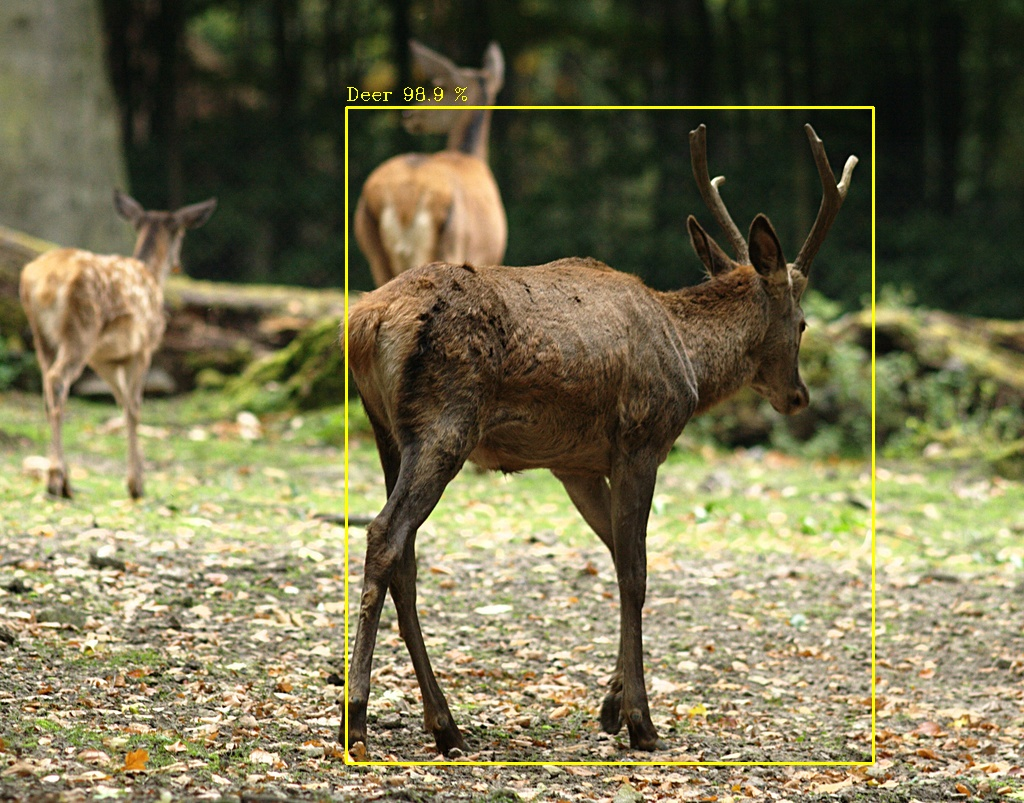
\includegraphics[width=0.9\textwidth]
  {model_compare_test__ssd_inception_v2.jpg}
  \captionof{figure}{SSD}
  \label{fig:infer_res_ssd}
\end{minipage}
\begin{minipage}{0.5\textwidth}
  \centering
  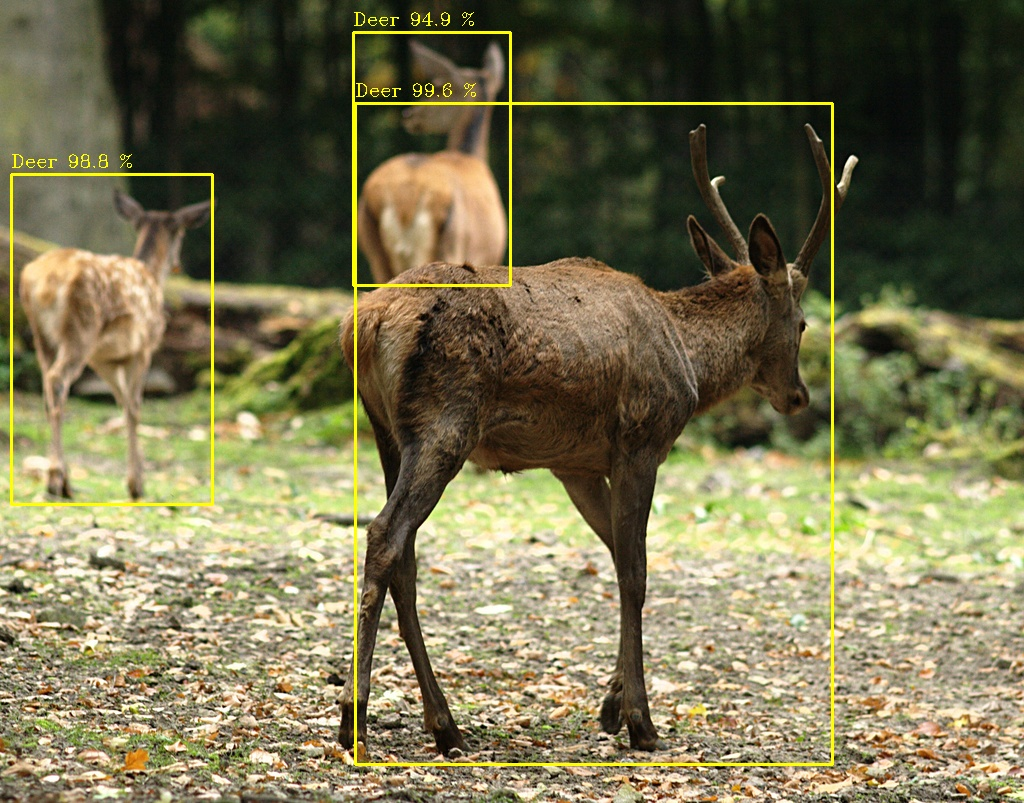
\includegraphics[width=0.9\textwidth]
  {model_compare_test__faster_rcnn_inception_v2_early_stopping.jpg}
  \captionof{figure}{Faster R-CNN}
  \label{fig:infer_res_faster_rcnn}
\end{minipage}


\subsubsection{Eigene Aufnahmen}

Bei der Inferenz, auf die eigenen Bilder, 
war ein deutlicher Unterschied der Modelle festzustellen.

In aufsteigender Reihenfolge lieferten das SSD mit MobilenetV2,
das SSD mit InceptionV2, das Faster R-CNN mit 
Early Stopping und Faster R-CNN mit Augmentierten Daten
wie in den Abbildungen \ref{fig:infer_res_ssd_mobile}
bis \ref{fig:infer_rest_rcnn_aug} zu sehen ist, 
bessere Ergebnisse.

Auch hier fiel auf, dass Tiere, die weiter weg und 
damit kleiner abgebildet sind,
besser von den Faster R-CNN Modellen
erkannt wurden.

\vspace{1cm}
\begin{minipage}{0.5\textwidth}
  \centering
  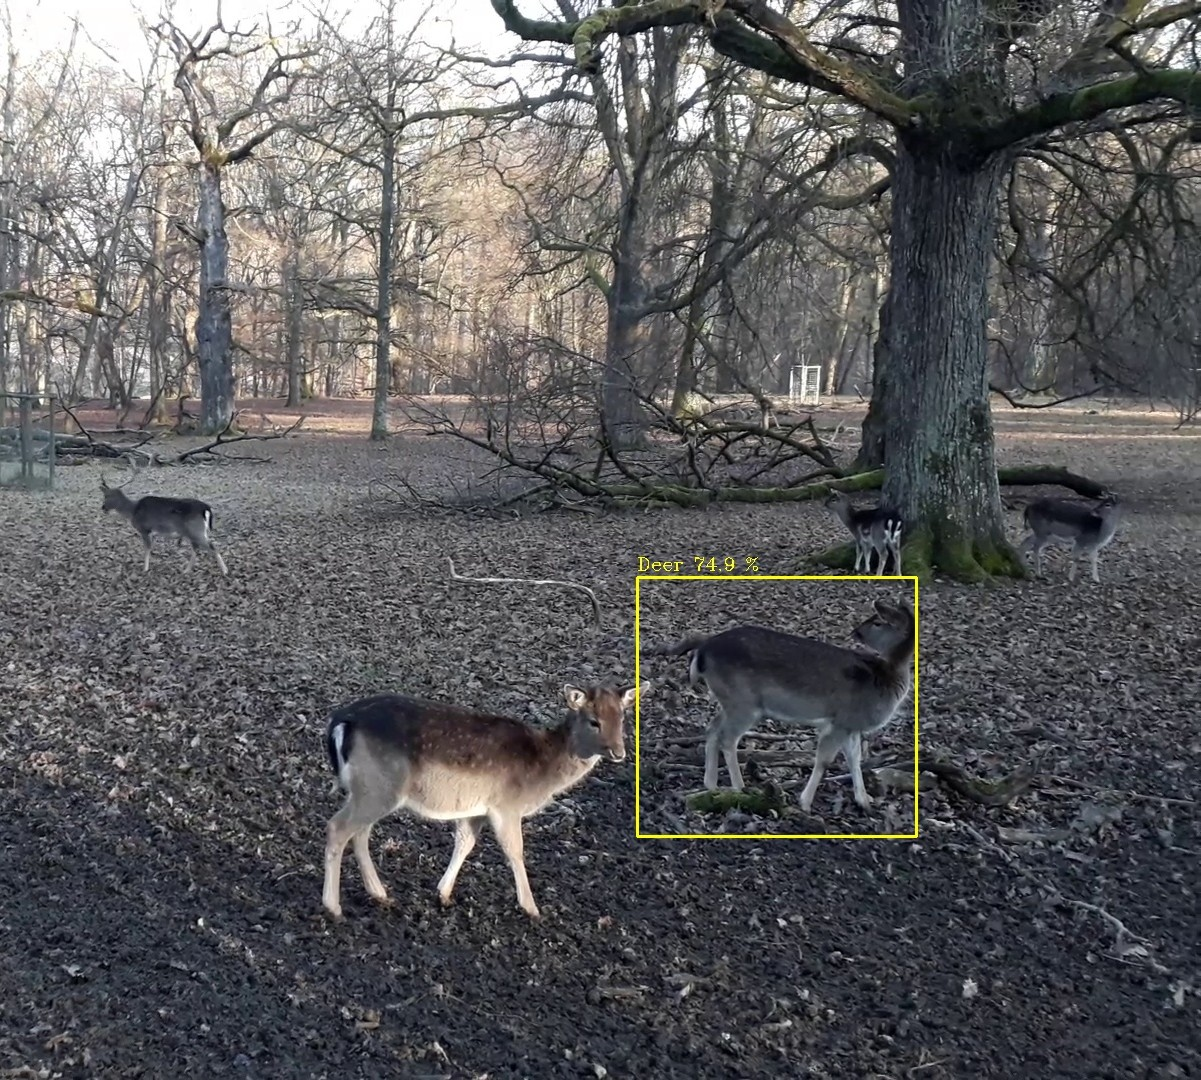
\includegraphics[width=0.9\textwidth]
  {model_compare_handy_ssd_mobilenet_v2.jpg}
  \captionof{figure}{SSD Mobilnet}
  \label{fig:infer_res_ssd_mobile}
\end{minipage}
\begin{minipage}{0.5\textwidth}
  \centering
  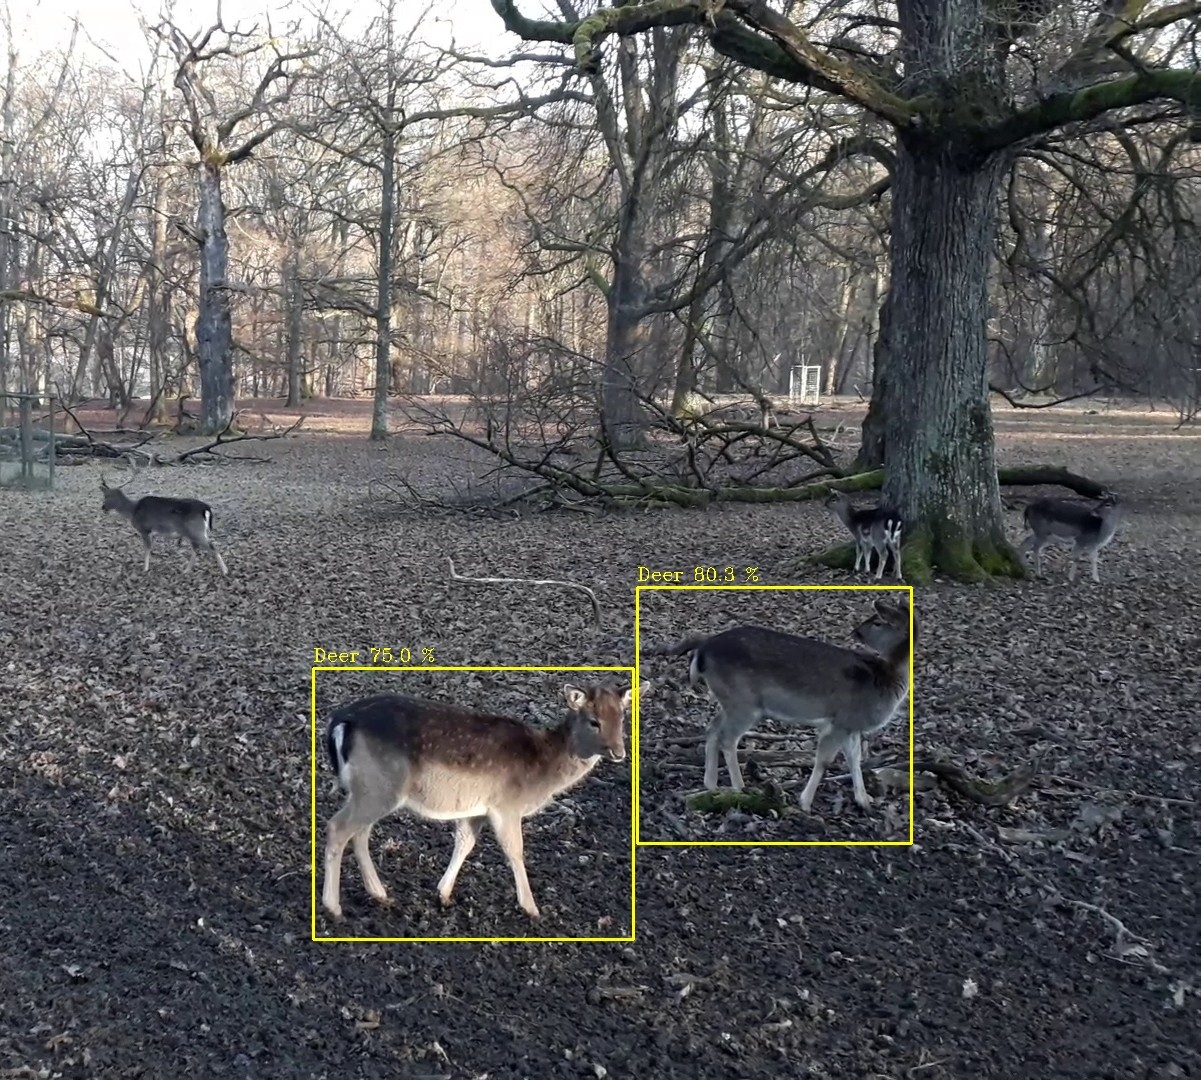
\includegraphics[width=0.9\textwidth]
  {model_compare_handy_ssd_inception_v2.jpg}
  \captionof{figure}{SSD Inception}
  \label{fig:infer_res_ssd_inception}
\end{minipage}
\\[1cm]
\begin{minipage}{0.5\textwidth}
  \centering
  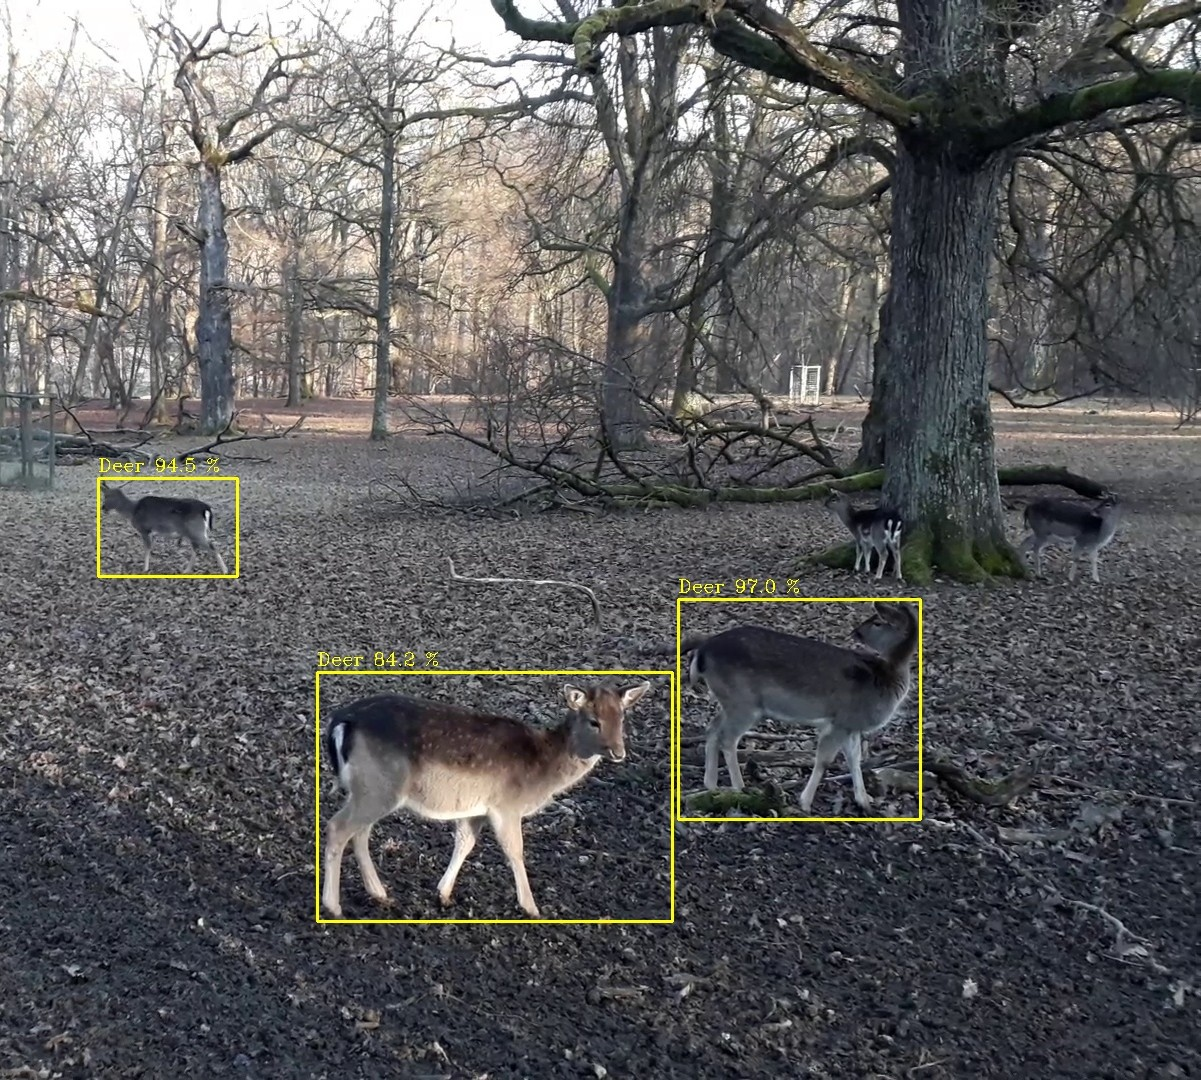
\includegraphics[width=0.9\textwidth]
  {model_compare_handy_faster_rcnn_inception_v2_early_stopping_ohne_aug.jpg}
  \captionof{figure}{Faster R-CNN mit Early Stopping}
  \label{fig:infer_res_rcnn_early_stopping}
\end{minipage}
\begin{minipage}{0.5\textwidth}
  \centering
  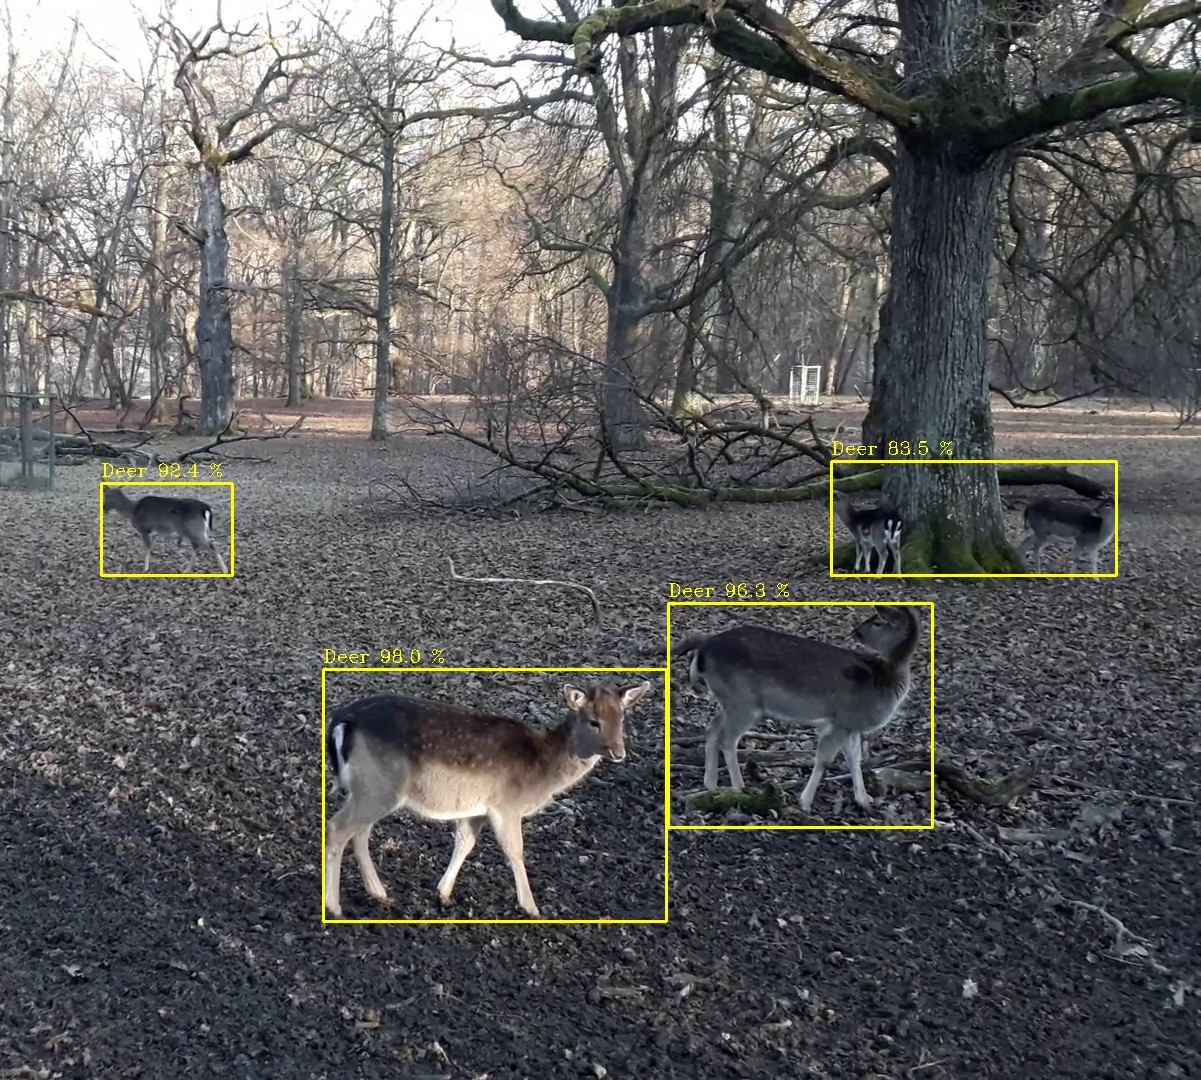
\includegraphics[width=0.9\textwidth]
  {model_compare_handy_faster_rcnn_inception_v2_early_stopping.jpg}
  \captionof{figure}{Faster R-CNN mit Augmentierung}
  \label{fig:infer_rest_rcnn_aug}
\end{minipage}



\subsubsection{iWildCam Datensatz}

Aus dem \textit{iWildCam 2019 Dataset}, welches aus einer 
\textit{Kaggle} Competition stammt, wurden die Klassen, welche
sich mit den für das Training verwendeten
überschnitten, für die Test Inferenz heruntergeladen.
Bei den Bildern handelt es sich um Aufnahmen von
Wildtier Kameras, aus dem Süd- und Nordwesten Amerikas,
welche aus der \textit{iNaturalist} und der \textit{Microsoft
DatAirSim} Datenbank stammen.

Darunter enthalten sind viele Nachtaufnahmen, welche teils 
schlecht beleuchtet und mit einer Infrarot Kamera aufgenommen und daher 
in Graustufen sind.

Da die Inferenzergebnisse hier bei allen vier Model Variationen 
deutlich schlechter, als bei den anderen Datensätzen war, 
wurde versucht dieses, durch weitere Optimierungen, zu verbessern.


%----------------- SECTION: optimierung ---------------------
\section{Optimierungen: Faster R-CNN}
\label{sec:optimierung_faster_rcnn}

Als Ausgangslage zur Verbesserung der Ergebnisse diente 
das Faster R-CNN mit augmentiertem Datensatz, welches
bei der Evaluierung im vorherigen Abschnitts die besten
Resultate erzielte.

Die Auswertung erfolgt hier wieder zunächst 
anhand der Evaluierungsmetriken und der Trainingsverläufe
aus Tensorboard und anschließend anhand der,
auf Testbilder ausgeführten, Inferenzergebnisse.



\subsection{Verschiedene Augmentierungen}

Der erste Ansatz zur Verbesserung der Ergebnisse war es,
das Faster R-CNN mit unterschiedlich starker Augmentierung
der Daten, für insgesamt mehr Iterationen
(500k statt 200k), zu trainieren.

Dabei wurde wieder das im Abschnitt \ref{subsec:augmentation} 
erläuterte Augmentierungsverfahren angewendetet, mit zusätzlich 
folgenden Variationen:

\begin{enumerate}
  \item Nur eine zufällige Augmentierung pro Bild, (anstelle von zwei)
  \item 4000 Bilder pro Klasse generieren (anstelle von 3000) 
\end{enumerate}

Die Trainingsergebnisse für 500k Iterationen sind anhand der 
Trainingsverläufe von Loss und mAP in den Abbildungen
\ref{plot:map_diff_aug} und \ref{plot:loss_diff_aug} dargestellt.

\vspace{1cm}
\begin{minipage}{0.5\textwidth}
  \centering
  \def\svgwidth{0.9\textwidth}
  \input{Bilder/plots/diff_aug_map.pdf_tex}
  \captionof{figure}{mAP}
  \label{plot:map_diff_aug}
\end{minipage}
\begin{minipage}{0.5\textwidth}
  \centering
  \def\svgwidth{0.9\textwidth}
  \input{Bilder/plots/diff_aug_loss.pdf_tex}
  \captionof{figure}{Loss}
  \label{plot:loss_diff_aug}
\end{minipage}

% Legende
% orange: FF7043
% blue  : 0077BB
% red   : CC3311
\begin{table}[htb]
  \centering
  \begin{tabular}{ m{0.4\textwidth}<{\centering}
                   m{0.2\textwidth}<{\centering}
                   m{0.2\textwidth}<{\centering}}
      $\color[HTML]{CC3311}\medbullet$ nur eine Augmentierung je Bild &
      $\color[HTML]{FF7043}\medbullet$  3000 Bilder &
      $\color[HTML]{0077BB}\medbullet$  4000 Bilder
  \end{tabular}    
\end{table}
\vspace{1cm}

Aufgrund des länger durchgeführten Trainings
ist bei allen Konfigurationen im, gegensatz zu den
Ergebnissen des vorherigen Abschnitts, Overfitting 
festzustellen.

Dieses fällt, wie zu erwarten war, bei den weniger  
augmentierten Datensätzen stärker aus, welche auf der 
anderen Seite einen besseren mAP Wert erreichen konnten.

Ob sich, konkret für diesen Fall, ein höherer mAP oder 
besserer Loss Wert positiver auf das Ergebnis auswirkt,
konnte wieder mithilfe der Inferenz auf Testbilder 
herausgefunnden werden.

\vspace{1cm}
\begin{minipage}{0.333\textwidth}
  \centering
  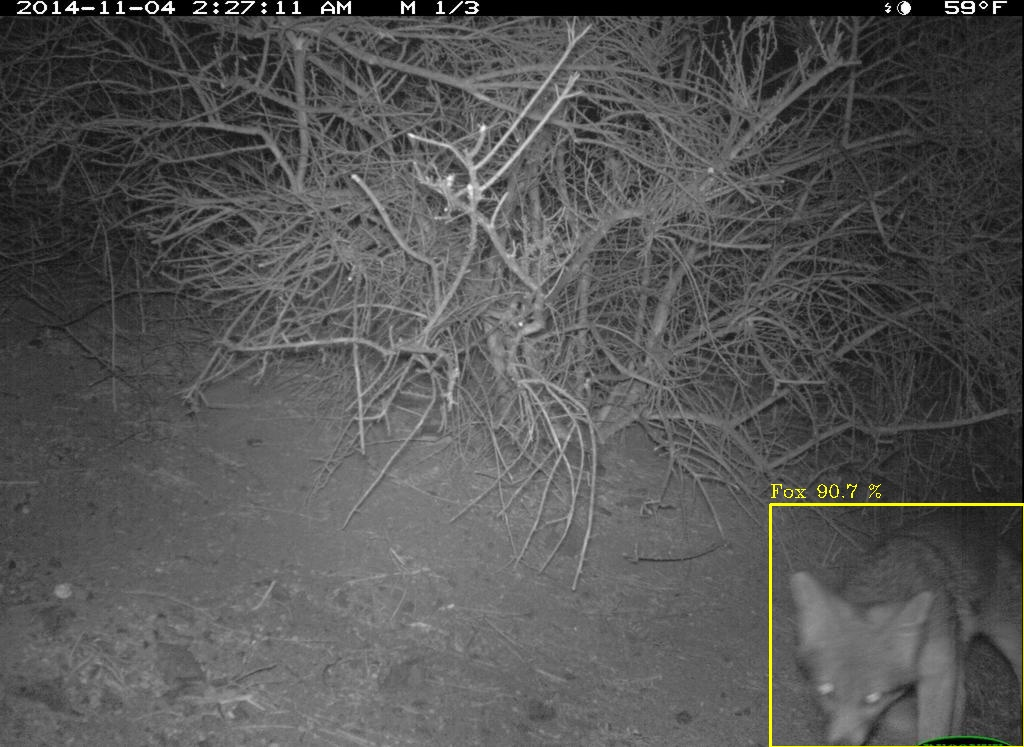
\includegraphics[width=\textwidth]{infer_images/iWildCam/fox/cut/59df5ee1-23d2-11e8-a6a3-ec086b02610b_faster_rcnn_inception_v2_3000.jpg}
  \captionof{figure}{3000 Samples}
  \label{fig:infer_res_3000}
\end{minipage}
\begin{minipage}{0.333\textwidth}
  \centering
  \label{fig:infer_res_4000}
  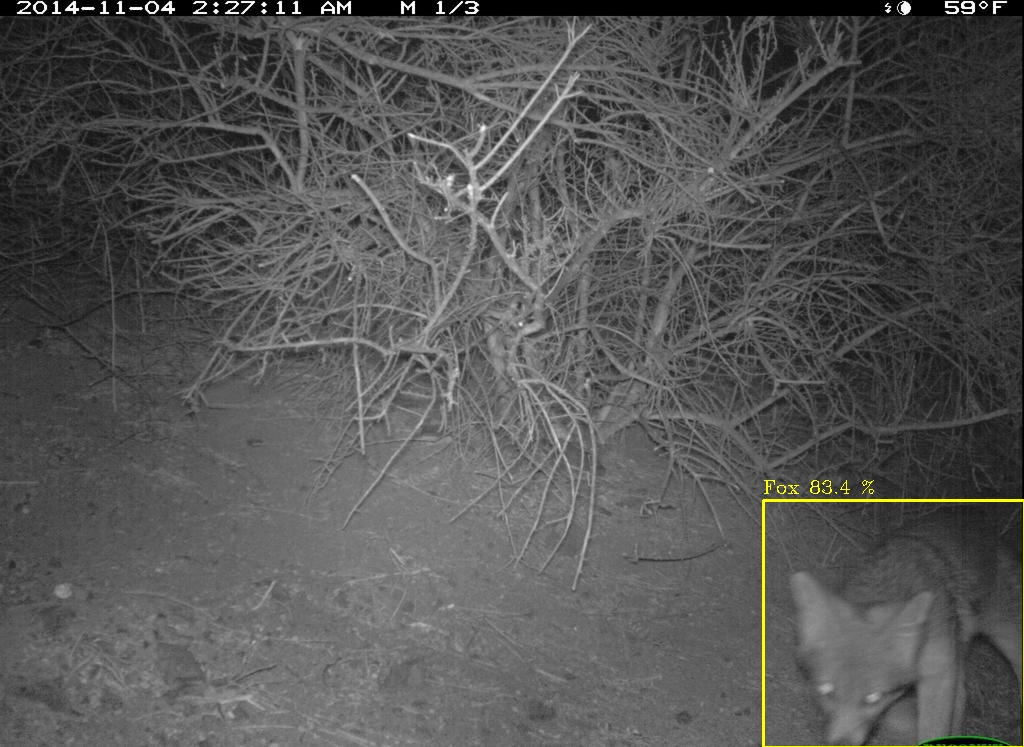
\includegraphics[width=\textwidth]{iWildCam/fox/cut/59df5ee1-23d2-11e8-a6a3-ec086b02610b_faster_rcnn_inception_v2_4000.jpg}
  \captionof{figure}{4000 Samples}
\end{minipage}
\begin{minipage}{0.333\textwidth}
  \centering
  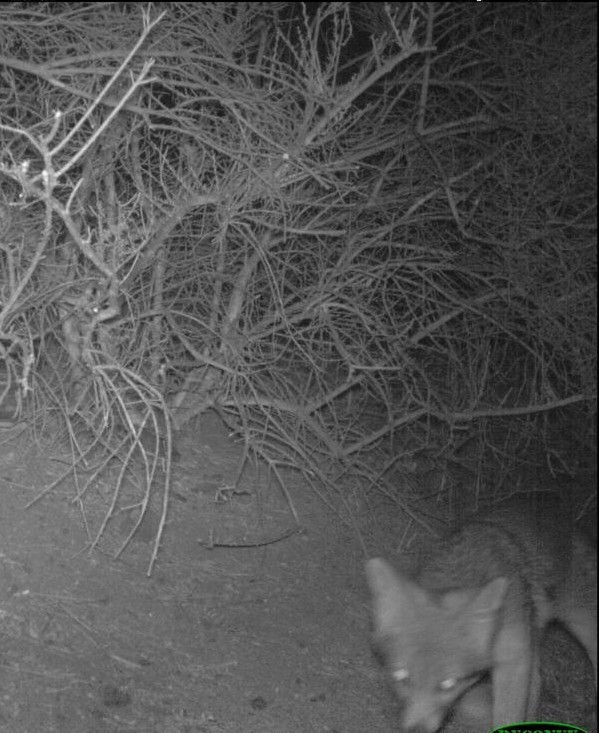
\includegraphics[width=\textwidth]{iWildCam/fox/cut/59df5ee1-23d2-11e8-a6a3-ec086b02610b_faster_rcnn_inception_v2_less_aug.jpg}
  \captionof{figure}{50\% Augment}
  \label{fig:infer_rest_05}
\end{minipage}
\vspace{1cm}

Abbildung \ref{fig:infer_res_3000} bis \ref{fig:infer_rest_05}
zeigen beispielhaft die Inferenzergebnisse für Bilder des 
\textit{iWildCam} Datensatzes, bei dem sich diesesmal der 
Unterschied deutlicher bemerkbar machte.
Das, auf weniger stark augmentierte Daten trainierte, 
Modell konnte die Tiere schlechter oder gar nicht erkennen.


\subsection{Verschiedene Regularisierungen}

Um das, trotz Augmentierung, zu stande kommende Overfitting zu 
vermeiden, wurde nun zusätzlich die L2 Regularisierung angewendet.
Diese soll, wie in den Grundlagen (Abschnitt \ref{subsec:validation})
beschrieben wurde, durch Anhängen einer Aufsummierung der Gewichte
an die Loss Funktion, ein Überanpassen des Modells an die
Trainingsdaten, reduzieren.

In der Konfigurationsdatei des Fater R-CNN kann dies,
durch setzten eines bestimmten Parameters für, sowohl die
erste Stufe des Modells, dem Region Proposal Network (RPN),
als auch für die zweite Stufe, dem Klassifikationsmodell,
seperat eingestellt werden.

Ebenso lassen sich die beiden Losskurven, aus denen sich 
beim Faster R-CNN der gesammte Loss zusammensetz,
seperat anzeigen, was in den Verläufen in 
Abbildung \ref{plot:aug_l2_classifier_loss}
und \ref{plot:aug_l2_rpn_loss} dargestellt ist.

Durch die getrennte Beobachtung der Loss-Kurven ließ sich 
feststellen, dass das Overfitting nur das RPN betrifft,
weshalb der Parameter zur L2 Regulierung nur 
für die erste Stufe eingestellt wurde.
Dafür wurde der Faktor $\lambda = 0.01$ gesetzt.

Vergleicht man nach dem Training mit 
reguliertem Modell wieder die Losskurven, ist deutlich zu 
erkennen, dass sich das Overfitting im RPN 
reduzieren ließ, wodurch sich auch der
in Abbildung \ref{plot:aug_l2_total_loss} 
dargestellte gesammt Loss verbesserte.

Die Verbesserung des Loss Wertes 
ging hier wieder mit einer leichten 
Verschlechterung des mAPs einher, wie in Abbildung
\ref{plot:aug_l2_mAP} zu erkennen ist.

\vspace{1cm}
\begin{minipage}{0.5\textwidth}
  \centering
  \def\svgwidth{0.9\textwidth}
  \input{Bilder/plots/aug_l2_mAP.pdf_tex}
  \captionof{figure}{mAP}
  \label{plot:aug_l2_mAP}
\end{minipage}
\begin{minipage}{0.5\textwidth}
  \centering
  \def\svgwidth{0.9\textwidth}
  \input{Bilder/plots/aug_l2_total_loss.pdf_tex}
  \captionof{figure}{Total Loss}
  \label{plot:aug_l2_total_loss}
\end{minipage}
\\[1cm]
\begin{minipage}{0.5\textwidth}
  \centering
  \def\svgwidth{0.9\textwidth}
  \input{Bilder/plots/aug_l2_classifier_loss.pdf_tex}
  \captionof{figure}{Klassifikations Loss}
  \label{plot:aug_l2_classifier_loss}
\end{minipage}
\begin{minipage}{0.5\textwidth}
  \centering
  \def\svgwidth{0.9\textwidth}
  \input{Bilder/plots/aug_l2_rpn_loss.pdf_tex}
  \captionof{figure}{RPN Loss}
  \label{plot:aug_l2_rpn_loss}
\end{minipage}
\begin{table}[htb]
  \centering
  \begin{tabular}{m{0.3\textwidth}<{\centering}
                  m{0.4\textwidth}<{\centering}}
     $\color[HTML]{CC3311}\medbullet$  nur Augmentierung &
     $\color[HTML]{0077BB}\medbullet$  Augmentierung + L2 Regularisierung
  \end{tabular}    
\end{table}
\vspace{1cm}

Auch hier wurde, zur Feststellung der Auswirkung 
der Unterschielichen Ergebnisse, wieder die 
Testinferenz angewendet, was beispielhaft 
für Bilder der eigenen Aufnahmen in den 
Abbildungen \ref{fig:test_infer_normal_aug}
und \ref{fig:test_infer_aug_plus_l2} dargestellt ist.


\vspace{1cm}
\begin{minipage}{0.5\textwidth}
  \centering
  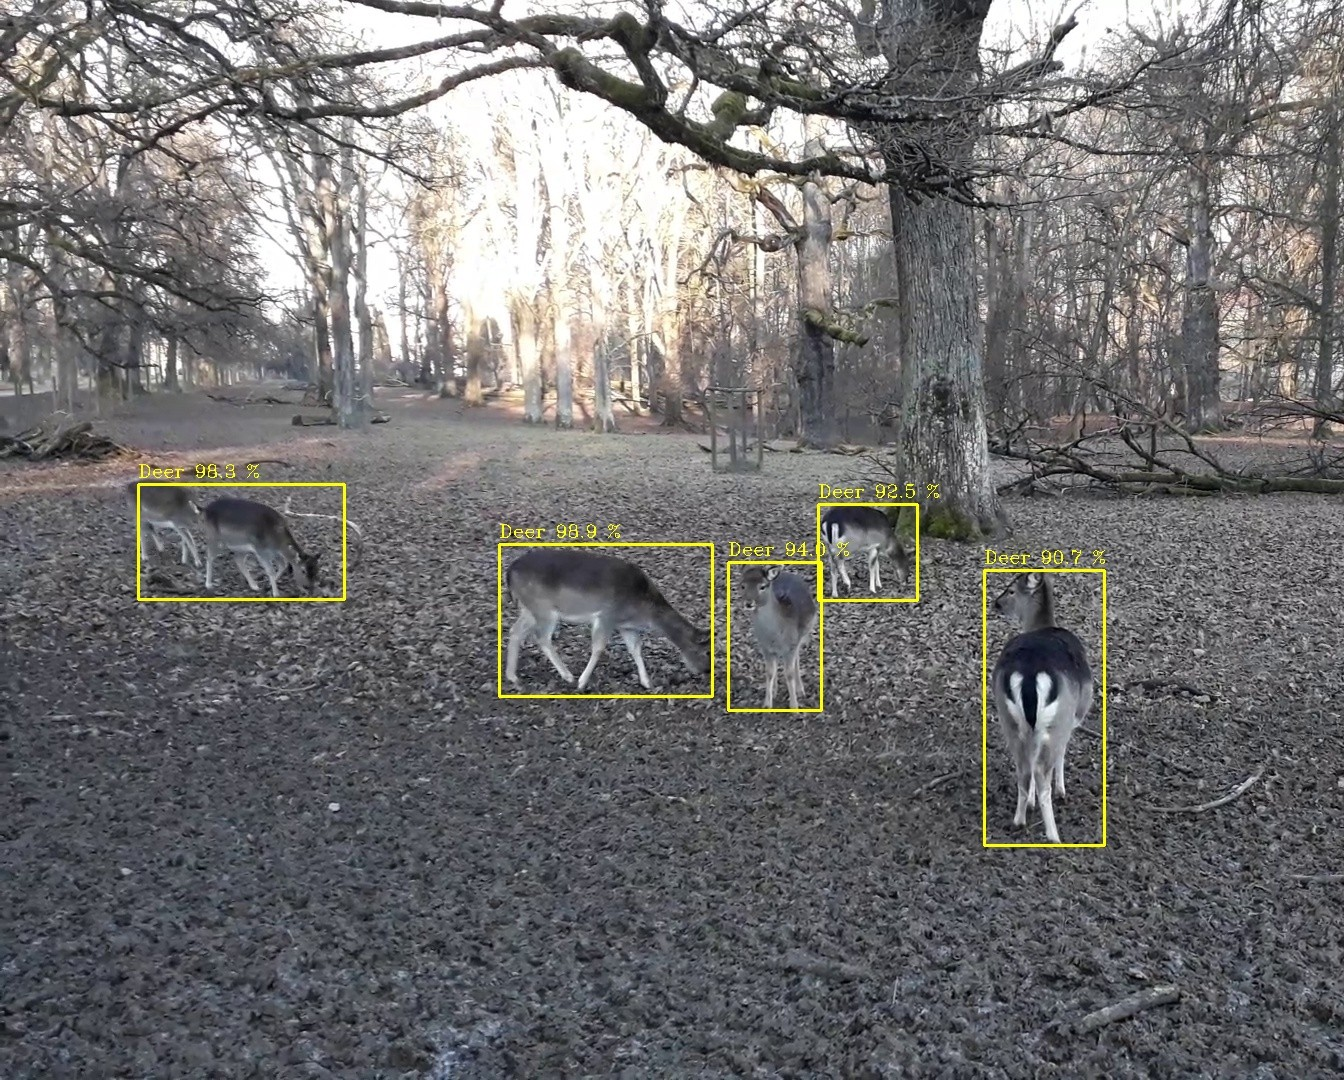
\includegraphics[width=0.95\textwidth]
  {eigene/20191229_145616_frame_20_faster_rcnn_inception_v2_3000.jpg}
  \captionof{figure}{Augmentierung (normal)}
  \label{fig:test_infer_normal_aug}
\end{minipage}
\begin{minipage}{0.5\textwidth}
  \centering
  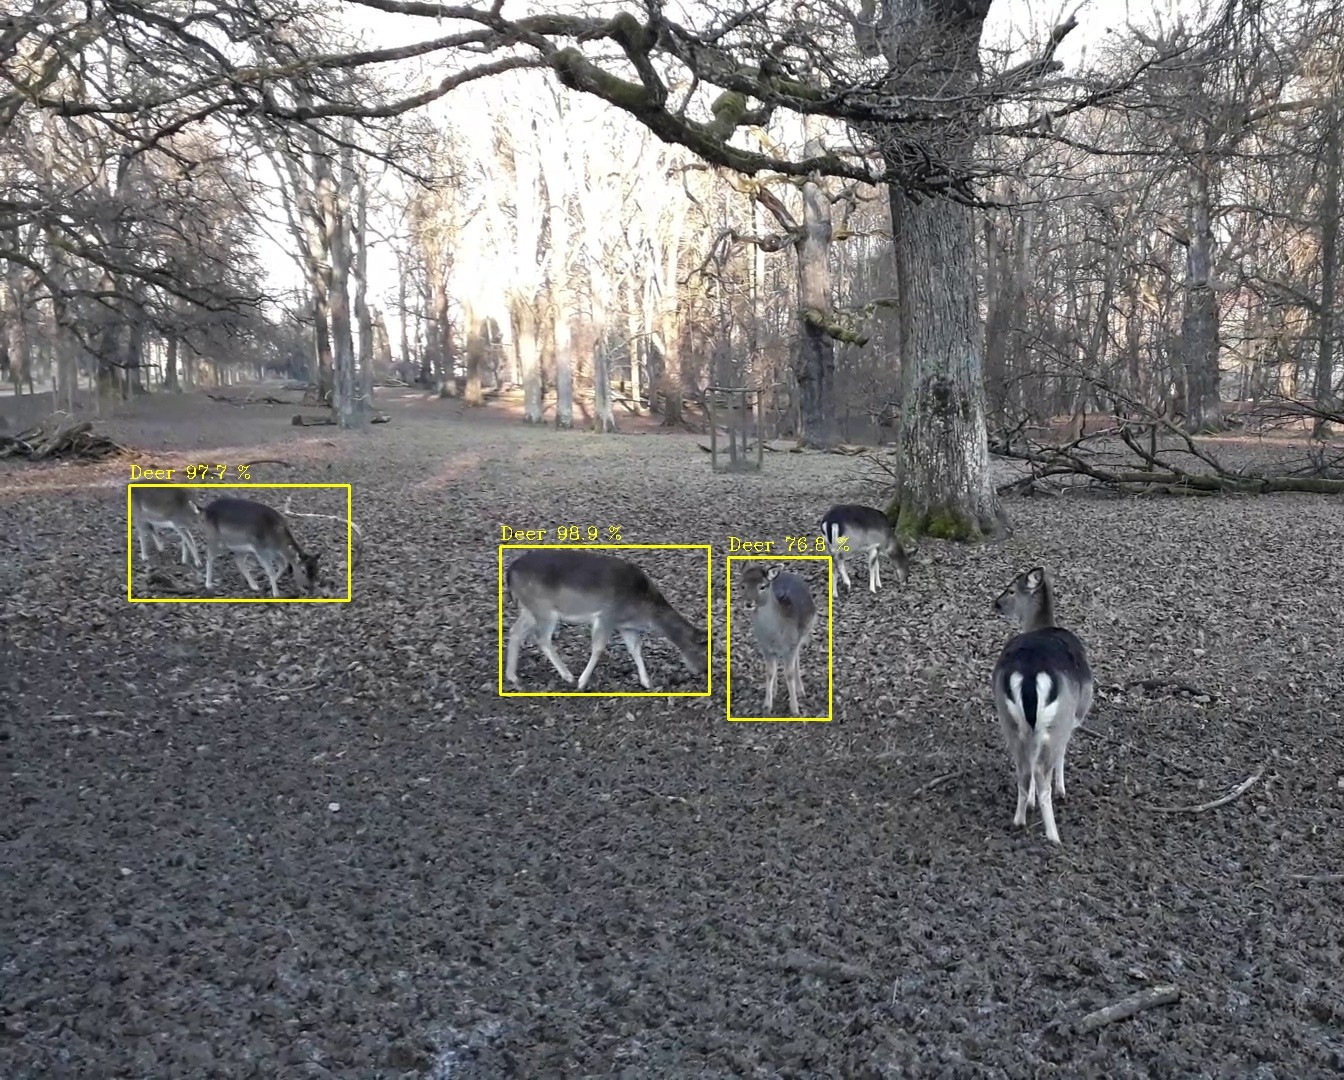
\includegraphics[width=0.95\textwidth]
  {eigene/20191229_145616_frame_20_faster_rcnn_inception_v2_l2.jpg}
  \captionof{figure}{Augmentierung + L2}
  \label{fig:test_infer_aug_plus_l2}
\end{minipage}
\vspace{1cm}

Hier ergaben die Inferenzergebnisse, dass 
eine L2 Regulierung der Modelle
in den meisten Fällen keinen Einfluss auf das Ergebnis
hat, falls doch, dieses sich tendentiell sogar
verschlechterte.

Weitere angewendete Regularisierungen, die jedoch 
auch zu keiner nennenswerten Veränderung der Trainingsergebnisse
führten, waren Dropout sowie L2 mit $\lambda = 0,02$ und sind in 
Tabelle \ref{table:reg}, zusammen mit den anderen Ergebnissen
dargestellt.


\vspace{1cm}
\begin{table}[htb]
  \centering
  \begin{tabular}{m{0.35\textwidth}|m{0.25\textwidth}<{\centering}m{0.25\textwidth}<{\centering}}
  \hline
                    & mAP  & Loss  \\ \hline\hline
  Augmentierung (50\%) &  0,72    &    0,76   \\
   + L2 Reg. ($\lambda = 0,01$)            &   0,71     & 0,75       \\\hline
  Augmentierung (normal)     & 0,7  & 0,74            \\
  + Dropout          & 0,7  & 0,73            \\
  + L2 Reg. ($\lambda = 0,01$)    & 0,7  & 0,69            \\
  + L2 Reg. ($\lambda = 0,02$)    & 0,69 & 0,7             \\ \hline
  Augmentierung (4000 Samples) &0,7&0,71\\\hline
  \end{tabular}
  \caption{Regularisierungen}
  \label{table:reg}
\end{table}
\vspace{1cm}

Aus den Ergebnissen ließ sich schließen, dass die Art
der Aufbereitung der Daten den größeren Einfluss auf die Ergebnisse
haben und durch Anpassungen der Hyperparameter, wenn überhaupt,
nur noch geringfügige Optimierungen betrieben werden können.
So hat insgesammt das Faster R-CNN, mit 500k Trainingsiterationen 
auf Augmentierte Daten mit 3000 Bildern je Klasse, zu
den besten Ergebnissen, bezüglich Genauigkeit, geführt.


\section{Inferenzzeit}\label{sec:infertime}

Neben der Genauigkeit, war die Ausführungszeit, welche ein Model für die 
Inferenz benötigt, ein weiteres Kriterium für die Auswahl des, in 
der Anwendung zu verwendenen, Modells.
Einer der Faktoren, welcher die Inferenzzeit beeinflusst,
ist die Hardware, auf der die Inferenz stattfindet,
sowie die zur Implementierung verwendeten Library.

Die Hardware war mit dem Neural Compute Stick 2 festgelegt, als 
Library kommen dafür \textit{OpenCV} oder \textit{OpenVino}
in Frage, wobei mit \textit{OpenVino} die Möglichkeit 
zur asynchronen Inferenzausführung, sowie der Verwendung mehrerer,
parallel ausgeführter, Inferenz Requests besteht,
wodurch sich die Inferenzzeit optimieren lässt.

Ein weiter Faktor ist die Komplexität des CNNs sowie die 
für die Objekterkennung verwendete Modell Architektur.
Üblicherweise sind Komplexere Modelle, wie das Faster R-CNN,
zwar genauer, jedoch auch langsamer.

Um den Effekt, den die drei unterschiedlichen, 
für das Training verwendeten, Varianten SSD mit MobilenetV2, 
SSD mit InceptionV2 und Faster R-CNN mit InceptionV2 auf die
Inferenzzeit haben zu Untersuchen,
wurden diese durch Messen der Inferenz-FPS verglichen.

Dabei wurde die Asynchrone Inferenz mit unterschiedlicher Anzahl 
an Inferenz Requests verwendet, weshalb in diesem Abschnitt 
zunächst die Funktionsweise der synchronen- und asynchronen
Inferenzausfürung mit OpenVino erklärt wird.


\subsection{Synchrone- und Asynchrone Inferenz}

Wird die Inferenz im synchronen Modus ausgeführt, kann immer
nur entweder inferiert, oder das Vor- und 
Nachverarbeiten, der Bilder stattfinden.

Vorverarbeitung der Bilder beeinhaltet dabei
z.B. die Umwandlung des von der Kamera gelieferten 
Bildformats, in das für das jeweilige Model richtige 
Input Format.
Die Nachverarbeitung bezieht sich auf das Verwenden 
der Inferenz Ergebnisse in der Anwendung.

Die Implementierung der Inferenz in OpenVino erfolgt
dementsprechend Sequentiell, wie im Algorithmus
\ref{code:sync} als Pseudocode dargestellt ist.

Anhand des zeitlichen Ablaufs, dargestellt in Abbildung
\ref{fig:sync}, sind die Abschnitte, in denen
keine Inferez stattfinden kann, deutlich zu erkennen.

\vspace{1cm}
\begin{minipage}{0.1\textwidth}
  \hfill
\end{minipage}
\begin{minipage}{0.5\textwidth}
  \begin{algorithm}[H]
    \caption{Synchrone Inferenz}
    \label{code:sync}
    \begin{algorithmic}
    \WHILE{\TRUE}
        \STATE capture FRAME
        \STATE preprocess CURRENT InferRequest
        \STATE \textbf{start} CURRENT InferRequest
        \STATE \textbf{wait} for CURRENT InferRequest
        \STATE process CURRENT result
    \ENDWHILE
    \end{algorithmic}
  \end{algorithm}  
\end{minipage}
\begin{minipage}{0.4\textwidth}
  \centering
  \vspace{1cm}
  \def\svgwidth{0.5\textwidth}
  \input{Bilder/sy_asy_legend.pdf_tex}
\end{minipage}

\vspace{1cm}
\begin{figure}[H]
  \centering
  \def\svgwidth{0.9\textwidth}
  %\tikzset{
    desicion/.style={
        diamond,
        draw,
        text width=4em,
        text badly centered,
        inner sep=0pt
    },
    block/.style={
        rectangle,
        draw,
        text width=5em,
        text height=1em,
        text centered
    },
    arrow/.style={
        draw,
        >=latex,
        ->
    }
}


\begin{tikzpicture}

    \node(infer1) [block] {infer1};
    \draw[arrow] (0,-1em) -- (10,-1em);
    % \node (A) [desicion] {entschei\\dung};
    % \node (B) [block, below of=A, node distance=5cm, text width=5em] {bock};
    % \node (C) [block, right of=A, node distance=5cm] {noch ein\\bock};


    % \draw[arrow] (A) --  node [left, fill=white] {yes} (B);
    % \draw[arrow] (A) -- node [below, near end] {crap} (C); 
    % \draw[arrow] (B) -| node [near start, fill=white] {yes} (C);

\end{tikzpicture}

  \input{Bilder/sync_infer.pdf_tex}
  \caption{}
  \label{fig:sync}
\end{figure}


Da die Inferenz auf dem Myriad Chip des Neural Compute Sticks
und nicht auf dem ausführenden Pc bzw. Raspberry Pi läuft,
kann diese ungehindert, parallel zum restlichen Programmablauf, 
erfolgen.

In OpenVino wird dieser Ablauf mithilfe der \textit{Asynchronen Api}
erreicht, welche, über einen bestimmten Funktionsaufruf,
die Inferenz in einem seperaten Thread startet.

Indem vor Erhalt und Verarbeitung eines aktuellen 
Inferenz Ergebnisses der Inferenz Request für
den nächsten Durchlauf aufgegeben wird, wie in Algorithmus
\ref{code:async} als Pseudocode dargestellt ist, kann der in
Abbildung \ref{fig:async} dargestellte Zeitliche Ablauf erreicht werden.


\vspace{1cm}
\begin{minipage}{0.1\textwidth}
  \hfill
\end{minipage}
\begin{minipage}{0.5\textwidth}
  \begin{algorithm}[H]
    \caption{Asynchrone Inferenz}
    \label{code:async}
    \begin{algorithmic}
    \WHILE{\TRUE}
        \STATE capture FRAME
        \STATE preprocess NEXT InferRequest
        \STATE \textbf{start} NEXT InferRequest
          \STATE \textbf{wait} for CURRENT InferRequest
          \STATE process CURRENT result
          \STATE swap CURRENT and NEXT InferRequest
    \ENDWHILE
    \end{algorithmic}
  \end{algorithm}
\end{minipage}
\begin{minipage}{0.4\textwidth}
  \centering
  \vspace{1cm}
  \def\svgwidth{0.5\textwidth}
  \input{Bilder/sy_asy_legend.pdf_tex}
\end{minipage}

\vspace{1cm}

\begin{figure}[H]
  \centering
  \def\svgwidth{0.9\textwidth}
  \input{Bilder/async_infer.pdf_tex}
  \caption{}
  \label{fig:async}
\end{figure}

Die hier mit \textit{Current} und \textit{Next} bezeichneten 
Inferenz Requests stehen für die Indizes der jeweiligen Requests
und können belieb erweitert werden. 
Dadurch wird erreicht, dass die Inferenz auf mehreren Threads 
parallel ausgeführt wird.
% https://docs.openvinotoolkit.org/2018_R5/_samples_object_detection_demo_ssd_async_README.html


\subsection{Vergleich der Modelle}

Mithilfe eines Python Scripts, in welchem die Asynchrone Inferenz 
für eine variabel einstellbare Anzahl an Inferenz Requests
implementiert wurde, konnte für die drei Modelle die 
durchschnittliche Anzahl an, pro Sekunde inferierten, Frames 
ermittelt werden.

Diese wurden auf dem Raspberry Pi mit dem Neural Compute Stick 
ausgeführt und lieferten die in Tabelle \ref{table:infertime}
dargestellten Ergebnisse.

\vspace{1cm}
\begin{table}[htb]
  \centering
  \begin{tabular}{m{0.25\textwidth}|m{0.1\textwidth}<{\centering}|m{0.1\textwidth}<{\centering}|m{0.1\textwidth}<{\centering}|m{0.1\textwidth}<{\centering}}
  \hline
  \multirow{2}{*}{Model} & \multicolumn{4}{c}{Asynchronge Inferenz Requests} \\ \cline{2-5} 
                         & 1           & 2          & 3          & 4          \\ \hline\hline
  SSD MobilenetV2        & 19,5           & 35,2          & 40,6          & 40,3          \\
  SSD InceptionV2        & 15,6           & 27,7          & 31,1          & 31,7          \\
  Faster R-CNN Incept.   & 0,63           & 0,67          & 0,75          & 0,74          \\ \hline
  \end{tabular}
  \caption{Vergleich von Inferenzzeiten der Modelle in FPS}
  \label{table:infertime}
\end{table}
\vspace{1cm}

Die asynchrone Inferenzausführung führte bei allen Modellen, 
für bis zu 3 inferenz Requests, zu besseren Ergebnissen.
Ein deutlicher Unterschied der Inferenzzeit war 
zwischen SSD und Faster R-CNN Architekuren festzustellen.

Da für die Anwendung zur Wildtiererkennung 
keine Realtime Performance erforderlich ist,
wurde durch geschickte Implementierung der Inferenz in der 
Applikation, trotz langsamerer Inferenzzeit, das 
Faster R-CNN verwendet.
